\section{Hiện tượng phóng xạ}
\subsection{Tóm tắt lí thuyết}
\begin{tomtat}
	\subsubsection{Hiện tượng phóng xạ}
	\paragraph{Định nghĩa}
	\begin{dn}
		Hiện tượng một hạt nhân không bền vững tự phát phân rã, phát ra các tia phóng xạ và biến đổi thành một hạt nhân khác.
	\end{dn}
	Quy ước:
	\begin{itemize}
		\item Hạt nhân phóng xạ là \textbf{hạt nhân mẹ};
		\item Hạt nhân sản phẩm của quá trình phân rã là \textbf{hạt nhân con}.
	\end{itemize}
	\paragraph{Các tính chất cơ bản của hiện tượng phóng xạ}
	Hiện tượng phóng xạ có hai tính chất cơ bản:
	\begin{itemize}
		\item \textbf{Tính tự phát:} quá trình phân rã xuất phát từ những biến đổi bên trong hạt nhân, hoàn toàn không phụ thuộc vào tác động bên ngoài (nhiệt độ, áp suất, \dots).
		\item \textbf{Tính ngẫu nhiên:} Với một hạt nhân phóng xạ cho trước, ta không thể xác định thời điểm phân rã của nó.
	\end{itemize}
	\subsubsection{Bản chất của các tia phóng xạ}
	\paragraph{Tia alpha $\left(\alpha\right)$}
	Tia $\alpha$ là dòng các hạt nhân $\ce{^4_2He}$, mang hai điện tích dương. Tia $\alpha$:
	\begin{itemize}
		\item bị lệch trong điện trường;
		\item có tốc độ khoảng $\SI{2E7}{\meter/\second}$;
		\item làm ion hoá các nguyên tử trên đường đi nên mất năng lượng nhanh và chỉ đi được tối đa $\SI{8}{\centi\meter}$ trong không khí;
		\item có tính đâm xuyên yếu, có thể bị chặn bởi tờ giấy có bề dày khoảng $\SI{1}{\milli\meter}$;
		\item gây nguy hiểm khi trực tiếp phóng xạ trong cơ thể người;
		\item phương trình phóng xạ: $\ce{^A_ZX}\longrightarrow\ce{^{A-4}_{Z-2}Y}+\ce{^4_2He}$.
	\end{itemize}
	\paragraph{Tia beta $\left(\beta\right)$}
	Tia $\beta$ có 2 loại:
	\begin{itemize}
		\item $\beta^-$ là dòng các electron $\ce{^0_{-1}e}$ mang điện tích âm;
		\item $\beta^+$ là dòng các positron $\ce{^0_{+1}e}$ mang điện tích dương.
	\end{itemize}
	Tia $\beta$ có các đặc điểm sau:
	\begin{itemize}
		\item bị lệch nhiều trong điện trường hơn tia $\alpha$;
		\item có tốc độ gần bằng tốc độ ánh sáng;
		\item làm ion hoá môi trường yếu hơn tia $\alpha$ nên đi được quãng đường dài hơn (vài mét) trong không khí;
		\item có tính đâm xuyên mạnh hơn tia $\alpha$;
		\item có cường độ lớn, có thể gây bỏng;
		\item trong phân rã $\beta$ còn xuất hiện hạt neutrino $\left(\nu\right)$ và phản hạt neutrino $\left(\overline{\nu}\right)$. Các hạt này không mang điện, khối lượng rất nhỏ và chuyển động với tốc độ xấp xỉ tốc độ ánh sáng;
		\item phương trình phóng xạ:
		\begin{itemize}
			\item phóng xạ $\beta^-$: $\ce{^A_ZX}\longrightarrow\ce{^A_{Z+1}Y}+\ce{^0_{-1}e}+\overline{\nu}$;
			\item phóng xạ $\beta^+$: $\ce{^A_ZX}\longrightarrow\ce{^A_{Z-1}Y}+\ce{^0_{+1}e}+\nu$;
		\end{itemize}
	\end{itemize}
	\paragraph{Tia gamma $\left(\gamma\right)$}
	Tia $\gamma$ là sóng điện từ có bước sóng rất ngắn $\left(\lambda<\SI{E-11}{\meter}\right)$, là chùm photon có năng lượng cao. Tia $\gamma$:
	\begin{itemize}
		\item không bị lệch trong điện trường;
		\item có tính đâm xuyên rất mạnh, lớn hơn nhiều so với $\alpha$ và $\beta$;
		\item ion hoá không khí mạnh;
		\item thường là tia phóng xạ kèm theo các tia $\alpha$ và $\beta$ khi hạt nhân con ở trạng thái năng lượng kích thích chuyển về trạng thái năng lượng cơ bản.
	\end{itemize}
	\begin{center}
		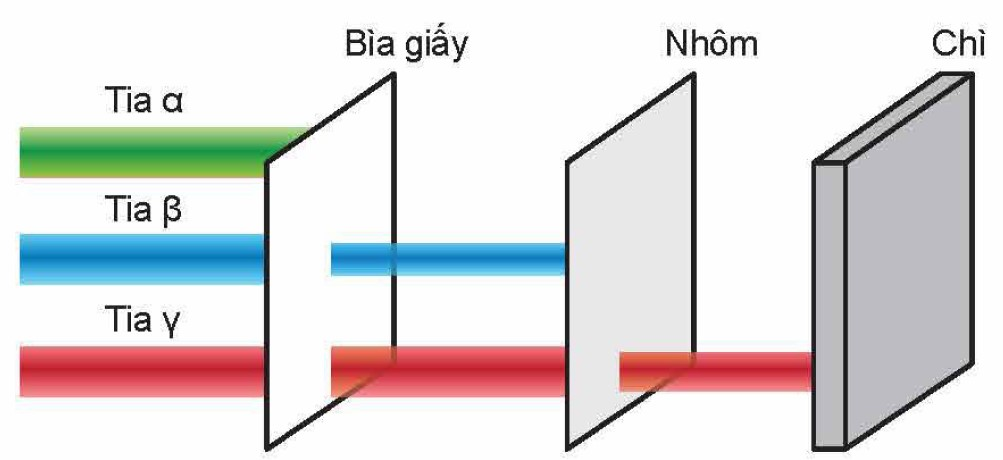
\includegraphics[width=0.5\linewidth]{figs/VN12-Y24-PH-SYL-031-4}
		\captionof{figure}{Minh họa khả năng đâm xuyên của các tia phóng xạ qua vật chất.}
	\end{center}
	\subsubsection{Định luật phóng xạ}
	\paragraph{Chu kỳ bán rã, hằng số phóng xạ}
\begin{boxdl}
		Cứ sau một khoảng thời gian xác định $T$ thì một nửa số hạt nhân hiện có sẽ bị phân rã, biến đổi thành hạt nhân khác; $T$ được gọi là chu kì bán rã của chất phóng xạ.\\
	Hằng số phóng xạ đặc trưng cho từng chất phóng xạ, có mối liên hệ với chu kì bán rã theo công thức:
	\begin{equation}
		\lambda=\dfrac{\ln 2}{T}.
	\end{equation}
\end{boxdl}
	trong đó:
	\begin{itemize}
		\item $\lambda$: hằng số phóng xạ, đơn vị trong hệ SI là $\si{\second^{-1}}$;
		\item $T$: chu kì bán rã, đơn vị trong hệ SI là $\si{\second}$.
	\end{itemize}
	\paragraph{Định luật phóng xạ}
	\begin{dl}
		Trong quá trình phân ra, số hạt nhân phóng xạ còn lại giảm theo thời gian theo quy luật hàm số mũ:
		\begin{equation}
			N_t=N_02^{-t/T}=N_0e^{-\lambda t}.
		\end{equation}
	\end{dl}
	trong đó:
	\begin{itemize}
		\item $N_t$: số hạt nhân còn lại;
		\item $N_0$: số hạt nhân ban đầu;
		\item $t$: thời gian phân rã, đơn vị trong hệ SI là $\si{\second}$;
		\item $T$: chu kì bán rã, đơn vị trong hệ SI là $\si{\second}$;
		\item $\lambda$: hằng số phóng xạ, đơn vị trong hệ SI là $\si{\second^{-1}}$. 
	\end{itemize}
	\subsubsection{Độ phóng xạ}
	\begin{dn}
		Độ phóng xạ là đại lượng đặc trưng cho tính phóng xạ mạnh hay yếu của một lượng chất phóng xạ, được xác định bằng số hạt nhân phóng xạ phân rã trong một giây.
		\begin{equation}
			H=-\dfrac{dN}{dt}=\lambda N
		\end{equation}
		Độ phóng xạ giảm theo thời gian với cùng quy luật hàm mũ giống số hạt nhân phóng xạ
		\begin{equation}
			H=H_0e^{-\lambda t}=H_02^{-t/T}
		\end{equation}
	\end{dn}
	Trong hệ SI, đơn vị của $H$ là becquerel $\left(\SI{1}{\becquerel}=\SI{1}{\text{phân rã}/\second}\right)$. Ngoài ra, $H$ còn có đơn vị là $\si{ci} \left(\SI{1}{ci}=\SI{3.66E10}{\becquerel}\right)$.
	\subsubsection{Quy tắc an toàn phóng xạ}
	Các quy tắc cơ bản cần thực hiện để đảm bảo an toàn khi ở các khu vực có nguồn phóng xạ hoặc phải làm việc trực tiếp với nguồn phóng xạ:
	\begin{itemize}
		\item Giảm thiểu thời gian tiếp xúc với nguồn phóng xạ.
		\item Giữ khoảng cách phù hợp đến nguồn phóng xạ.
		\item Sử dụng các màn chắn, trang phục bảo hộ để đảm bảo che chắn phóng xạ.
	\end{itemize}
\end{tomtat}
\subsection{Ví dụ minh hoạ}
\begin{dang}{Vận dụng các định luật bảo toàn trong phản ứng hạt nhân để viết đúng phương trình phân rã}
\end{dang}
\begin{vd}
	Uranium 238 sau một loạt phóng xạ $\alpha$ và biến thành chì. Phương trình của phản ứng là: $$\ce{^{238}_{92}U}\longrightarrow\ce{^{206}_{82}Pb}+x\ce{^4_2He}+y\ce{^0_{-1}\beta^{-}}.$$
	Xác định giá trị của $x$ và $y$.
	\loigiai{Bảo toàn điện tích và bảo toàn số khối, ta thu được hệ phương trình:
		\begin{align*}
			\begin{cases}
				4x+0y=238-206=32\\
				2x+\left(-1\right)y=92-82
			\end{cases}\Rightarrow\begin{cases}
				x=8\\
				y=6
			\end{cases}.
	\end{align*}}
\end{vd}
\begin{dang}{Vận dụng định luật phóng xạ xác định số hạt/khối lượng hạt nhân phóng xạ còn lại}
		Sau thời gian $t$, số hạt và khối lượng hạt nhân phóng xạ còn lại:
		\begin{equation}
			\begin{cases}
				N=N_02^{-t/T}=N_0e^{-\lambda t}\\
				m=m_02^{-t/T}=m_0e^{-\lambda t}
			\end{cases}.
		\end{equation}	
		Số hạt và khối lượng hạt nhân đã phóng xạ:
		\begin{equation}
			\begin{cases}
				\Delta N=N_0-N=N_0\left(1-2^{-t/T}\right)=N_0\left(1-e^{-\lambda t}\right)\\
				\Delta m=m_0-m=m_0\left(1-2^{-t/T}\right)=m_0\left(1-e^{-\lambda t}\right)
			\end{cases}
		\end{equation}
\end{dang}
\begin{vd}
Chất phóng xạ polonium $\ce{^{210}_{84}Po}$ phóng xạ tia $\alpha$ và biến thành hạt nhân chì $\ce{Pb}$. Biết chu kì bán rã của $\ce{^{210}_{84}Po}$ là 138 ngày và ban đầu có $\SI{100}{\gram}$ chất. Lấy khối lượng nguyên tử xấp xỉ số khối.
\begin{enumerate}[label=\alph*)]
	\item Tính số hạt $\ce{Po}$ và khối lượng $\ce{Po}$ còn lại sau 69 ngày.
	\item Tính số hạt $\ce{Po}$ bị phân rã và khối lượng $\ce{Po}$ đã phân rã sau 80 ngày.
	\item Sau 150 ngày có bao nhiêu phần trăm $\ce{Po}$ bị phân rã?
	\item Sau bao lâu $\ce{Po}$ bị phân rã $\SI{12.5}{\gram}$?
	\item Sau bao lâu (kể từ thời điểm ban đầu) số hạt nhân của $\ce{^{210}_{84}Po}$ phóng xạ còn lại bằng $\SI{25}{\percent}$ số hạt nhân ban đầu?
\end{enumerate}
\loigiai{
Số hạt nhân $\ce{Po}$ ban đầu có trong mẫu:
$$N_0=\dfrac{m}{A}N_A=\dfrac{\left(\SI{100}{\gram}\right)}{\left(\SI{210}{\gram/\mole}\right)}\cdot\left(\SI{6.02E23}{\mole^{-1}}\right)\approx\SI{2.866E23}{\text{hạt}}.$$
\begin{enumerate}[label=\alph*)]
	\item Sau 69 ngày, số hạt và khối lượng $\ce{Po}$ còn lại là:
	$$\begin{cases}
		N=N_0\cdot2^{-t/T}=\SI{2.866E23}{}\cdot 2^{-\frac{69}{138}}=\SI{2.027E23}{\text{hạt}}\\
		m=m_0\cdot 2^{-t/T}=\left(\SI{100}{\gram}\right)\cdot2^{-\frac{69}{138}}=\xsi{50\sqrt{2}}{\gram}
	\end{cases}.$$
	\item Sau 80 ngày, số hạt và khối lượng $\ce{Po}$ đã bị phân rã:
	$$\begin{cases}
		\Delta N=N_0\left(1-2^{-t/T}\right)=\SI{2.866E23}\cdot\left(1-2^{-\frac{80}{138}}\right)=\SI{9.48E22}{\text{hạt}}\\
		\Delta m=m_0\left(1-2^{-t/T}\right)=\left(\SI{100}{\gram}\right)\cdot\left(1-2^{-\frac{80}{138}}\right)\approx\SI{33.1}{\gram}
	\end{cases}.$$
	\item Sau 150 ngày, phần trăm $\ce{Po}$ bị phân rã là
	$$\dfrac{\Delta m}{m_0}=1-2^{-t/T}=1-2^{-\frac{150}{180}}=\SI{52.924}{\percent}.$$
	\item Khối lượng $\ce{Po}$ bị phân rã:
	$$\Delta m=m_0\left(1-2^{-t/T}\right)\Leftrightarrow 0,25=2^{-\frac{t}{138}}\Rightarrow t=\SI{276}{\text{ngày}}.$$
	\item Số hạt nhân $\ce{Po}$ phóng xạ còn lại $\SI{25}{\percent}$ so với ban đầu thì 
	$$\dfrac{N}{N_0}=2^{-t/T}\Leftrightarrow 0,25=2^{-\frac{t}{138}}\Rightarrow t=\SI{276}{\text{ngày}}.$$
\end{enumerate}
}
\end{vd}
% ======================================
\begin{vd}
	Hình bên biểu diễn sự phụ thuộc của số hạt còn lại và số hạt đã bị phân rã theo thời gian $t$ của một mẫu chất phóng xạ X.
	\begin{center}
		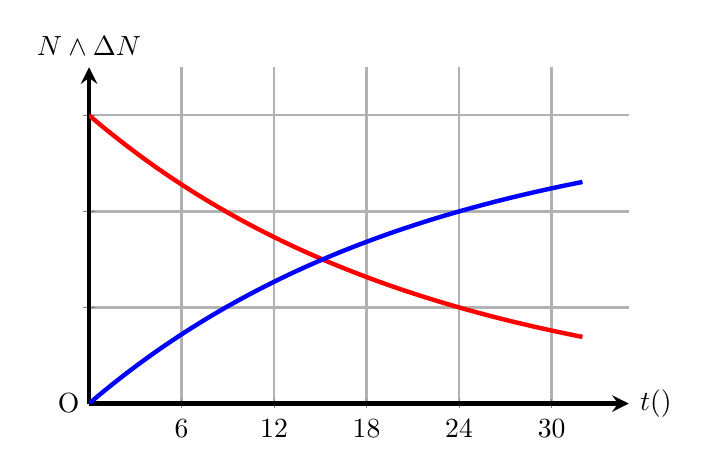
\begin{tikzpicture}  
			\begin{axis}[  ultra thick,yscale=0.75,
				xmin=0,  
				xmax=35,  
				xtick={0,6,...,30},
				ytick={0,1,2,3},
				yticklabels=\empty,
				minor x tick num=0,
				minor y tick num=0,
				ymin=0,  
				ymax=3.5, 
				samples=300,
				axis lines=center, 
				grid style={step=1, line width =0.4pt, color=gray!30!white},
				grid=both,
				major grid style={line width=0.8pt,gray!60!white},
				xlabel=$\xsi{t}{\left(\si{\hour}\right)}$, 		ylabel=$N\wedge\Delta N$,
				every axis y label/.style={at=(current axis.above origin),anchor=south},  
				every axis x label/.style={at=(current axis.right of origin),anchor=west},  ]
				\addplot [ultra thick, red, smooth, domain=0:32] {3*2^(-x/15.1423)};  
				\addplot [ultra thick, blue, smooth, domain=0:32] {3-3*2^(-x/15.1423)};
			\end{axis}  
			\node[left] at (0,0) {O};
		\end{tikzpicture}
		
	\end{center}
	\begin{enumerate}[label=\alph*)]
		\item Chu kì bán rã của X bằng bao nhiêu?
		\item Tại thời điểm $t=\SI{18}{\hour}$, số hạt X đã bị phân rã gấp mấy lần số hạt X còn lại trong mẫu?
	\end{enumerate}
	\loigiai{
	\begin{enumerate}[label=\alph*)]
		\item Dựa vào đồ thị, tại thời điểm $t=\SI{24}{\hour}$ thì
		$$\Delta N=2N\Leftrightarrow N_0\left(1-2^{-t/T}\right)=2N_0\cdot 2^{-t/T}\Leftrightarrow \left(1-2^{-\frac{24}{T}}\right)=2\cdot2^{-\frac{24}{T}}$$
		$\Rightarrow T\approx\SI{15.14}{\hour}.$
		\item Tại $t=\SI{18}{\hour}$:
		$$\dfrac{\Delta N}{N}=\dfrac{1-2^{-t/T}}{2^{-t/T}}=\dfrac{1-2^{-18/15,14}}{2^{-18/15,14}}\approx1,28.$$
		Vậy tại thời điểm $t=\SI{18}{\hour}$, số hạt X đã bị phân rã gấp 1,28 lần số hạt X còn lại.
	\end{enumerate}
	}
\end{vd}

\begin{dang}{Bài toán về số hạt nhân và khối lượng hạt nhân con tạo thành}
		Xét hạt nhân X phóng xạ ra tia phóng xạ C và biến đổi thành hạt nhân Y:
		\begin{equation}
			\ce{X}\longrightarrow \ce{Y}+\ce{C}
		\end{equation}
		Mỗi hạt nhân mẹ bị phân rã tạo thành một hạt nhân con nên số hạt nhân con tạo thành đúng bằng số hạt nhân mẹ bị phân rã:
		\begin{equation}
			\begin{cases}
				N_{\ce{Y}}=\Delta N_{\ce{X}}=N_{\ce{0X}}\left(1-2^{-t/T}\right)\\
				n_{\ce{Y}}=\Delta n_{\ce{X}}=n_{\ce{0X}}\left(1-2^{-t/T}\right)
			\end{cases}
		\end{equation}
		Khối lượng hạt nhân con Y được tạo thành sau thời gian $t$ là
		\begin{equation}
			n_{\ce{Y}}=n_{\ce{0X}}\left(1-2^{-t/T}\right)\Leftrightarrow \dfrac{m_{\ce{Y}}}{A_{\ce{Y}}}=\dfrac{m_0}{A_{\ce{X}}}\left(1-2^{-t/T}\right)\Rightarrow m_{\ce{Y}}=m_0\left(1-2^{-t/T}\right)\dfrac{A_{\ce{Y}}}{A_{\ce{X}}}
		\end{equation}
\end{dang}
\begin{vd}
	Chất polonium $\ce{^{210}_{84}Po}$ phóng xạ alpha $\left(\alpha\right)$ và chuyển thành chì $\ce{^{206}_{82}Pb}$ với chu kỳ bán rã là 138,4 ngày. Khối lượng ban đầu của $\ce{Po}$ là $\SI{50}{\gram}$.
	\begin{enumerate}[label=\alph*)]
		\item Sau 100 ngày (kể từ thời điểm ban đầu) thì tỉ số của số hạt nhân $\ce{Pb}$ và $\ce{Po}$ bằng bao nhiêu?
		\item Sau bao lâu khối lượng hạt nhân $\ce{Po}$ gấp 4 lần khối lượng hạt nhân $\ce{Pb}$?
	\end{enumerate}
	\loigiai{
	Phương trình phản ứng: $\ce{^{210}_{84}Po}\longrightarrow \ce{^4_2\alpha}+\ce{^{206}_{82}Pb}$.
	\begin{enumerate}[label=\alph*)]
		\item Sau 100 ngày (kể từ thời điểm ban đầu) thì tỉ số của số hạt nhân $\ce{Pb}$ và $\ce{Po}$ là
		$$\dfrac{N_{\ce{Pb}}}{N_{\ce{Po}}}=2^{t/T}-1=2^{\frac{100}{138,4}}-1\approx0,6524.$$
		\item Ta có:
		$$\dfrac{m_{\ce{Pb}}}{m_{\ce{Po}}}=\dfrac{A_{\ce{Pb}}}{A_{\ce{Po}}}\left(2^{t/T-1}\right)\Leftrightarrow \dfrac{1}{4}=\dfrac{206}{210}\left(2^{\frac{t}{138,4}}-1\right)\Rightarrow t=\SI{45.1977}{\text{ngày}}.$$
	\end{enumerate}	
	}
\end{vd}
	% ============================
	\begin{vd}
		Hạt nhân uranium $\ce{^{238}_{92}U}$ sau một chuỗi phân rã, biến đổi thành hạt nhân chì $\ce{^{206}_{82}Pb}$. Trong quá trình đó, chu kì bán rã của $\ce{^{238}_{92}U}$ biến đổi thành hạt nhân chì là $\SI{4.47E9}{\text{năm}}$. Một khối đá được phát hiện có chứa $\SI{1.188E20}{}$ hạt nhân $\ce{^{238}_{92}U}$ và $\SI{6.239E18}{}$ hạt nhân $\ce{^{206}_{82}Pb}$. Giả sử khối đá lúc mới hình thành không chứa hạt nhân chì và tất cả lượng hạt nhân chì có mặt trong đó đều là sản phẩm phân rã của $\ce{^{238}_{92}U}$. Tuổi của khối đá khi được phát hiện là bao nhiêu?
		\loigiai{
		Số hạt chì tạo thành bằng số hạt uranium đã phóng xạ: $N_{\ce{Pb}}	=\Delta N_{\ce{U}}$.\\
		Theo đề bài, ta có:
		$$\dfrac{N_{\ce{Pb}}}{N_{\ce{U}}}=\dfrac{\Delta N_{\ce{U}}}{N_{\ce{U}}}=\dfrac{N_0\left(1-2^{-t/T}\right)}{N_0\cdot2^{-t/T}}=2^{t/T}-1=\dfrac{\SI{6.239E18}{}}{\SI{1.188E20}{}}=0,0525.$$
		$$\Rightarrow2^{t/T}=1,0525\Rightarrow t=\SI{3.3E8}{\text{năm}}.$$
		Vậy tuổi của khối đá khi được phát hiện là $\SI{3.3E8}{\text{năm}}$.
		}
	\end{vd}
	\begin{dang}{Định nghĩa được độ phóng xạ, hằng số phóng xạ và vận dụng được mối liên hệ $H=\lambda N$}
	\end{dang}
	\begin{vd}
		Một mẫu chất phóng xạ $\beta^+$ là $\ce{^{15}_8O}$ có độ phóng xạ là $\SI{2.80E7}{\becquerel}$. Biết rằng hằng số phóng xạ của $\ce{^{15}_8O}$ là $\SI{5.67E-3}{\second^{-1}}$.
		\begin{enumerate}[label=\alph*)]
			\item Xác định số hạt nhân chất phóng xạ có trong mẫu khi đó.
			\item Xác định số hạt positron mẫu chất phát ra trong khoảng thời gian $\SI{1.00}{\milli\second}$. Coi gần đúng rằng độ phóng xạ của mẫu không thay đổi trong khoảng thời gian rất ngắn này.
		\end{enumerate}
		\loigiai{\begin{enumerate}[label=\alph*)]
				\item Số hạt nhân chất phóng xạ có trong mẫu khi đó:
				$$N_0=\dfrac{H_0}{\lambda}=\dfrac{\SI{2.80E7}{\becquerel}}{\SI{5.67E-3}{\second^{-1}}}\approx\SI{49.38E8}{\text{hạt}}.$$
				\item Trong quá trình phóng xạ trên diễn ra, mỗi hạt nhân bị phóng xạ sẽ phát ra một hạt positron. Do đó, số hạt positron mẫu chất phát ra bằng số hạt nhân $\ce{^{15}_8O}$ phân rã:
				$$N_{\beta^+}=\Delta N=N_0\left(1-e^{-\lambda t}\right)=\SI{49.38E8}{}\cdot\left[1-e^{-\left(\SI{5.67E-3}{\second^{-1}}\right)\cdot\left(\SI{1.00E-3}{\second}\right)}\right]\approx\SI{27998}{\text{hạt}}.$$
		\end{enumerate}}
	\end{vd}
% ===============================================
\begin{vd}
	Nhờ một máy đếm xung người ta có được thông tin sau về 1 chất phóng xạ. Ban đầu, trong thời gian 1 phút có 360 nguyên tử của chất phóng xạ, nhưng 2 giờ sau (kể từ thời điểm ban đầu) thì trong 1 phút chỉ có 90 nguyên tử phóng xạ. Tìm chu kì bán rã của chất phóng xạ này.
	\loigiai{
	Độ phóng xạ ban đầu: $H_0=\dfrac{360}{60}=\SI{6}{\becquerel}$.\\
	Độ phóng xạ sau 2 giờ: $H=\dfrac{90}{60}=\SI{1.5}{\becquerel}$.\\
	Từ $H=H_02^{-\frac{t}{T}}\Leftrightarrow 1,5=6\cdot 2^{-\dfrac{2}{T}}\Rightarrow T=\SI{1}{\hour}.$	
	}
\end{vd}
% ==================================
\begin{vd}
Một mẫu ban đầu chứa đồng vị $\ce{^{60}_{27}Co}$ nguyên chất, là chất phóng xạ $\gamma$ với chu kì bán rã $\SI{5.27}{\text{năm}}$ được sử dụng trong điều trị ung thư. Khi mẫu này được sử dụng lần đầu thì thời gian cho một liều chiếu xạ là 15 phút. Hỏi sau 2 năm, nếu vẫn sử dụng mẫu chất này thì thời gian cho một liều chiếu xạ là bao nhiêu? Coi như lượng hạt $\gamma$ cho một liều chiếu xạ trong cả hai lần là như nhau.
\loigiai{
Độ phóng xạ tại thời điểm ban đầu:
$$H_0=\dfrac{\Delta N_0}{\Delta t_0}$$
với $\Delta N_0$ là số hạt đã phân rã trong thời gian $\Delta t_0$.\\
Độ phóng xạ tại thời điểm $t$:
$$H=\dfrac{\Delta N}{\Delta t}$$
với $\Delta N$ là số hạt đã phân rã trong thời gian $\Delta t$.\\
Từ $H=H_0\cdot 2^{-\frac{t}{T}}\Rightarrow \dfrac{\Delta N}{\Delta t}=\dfrac{\Delta N_0}{\Delta t_0}\cdot 2^{-\frac{t}{T}}$.\\
Do liều chiếu xạ ở cả 2 lần là như nhau: $\Delta N_0=\Delta N\Rightarrow \Delta t=\Delta t_0\cdot 2^{\frac{t}{T}}=\left(\SI{15}{\minute}\right)\cdot2^{\frac{\SI{2}{\text{năm}}}{\SI{5.27}{\text{năm}}}}\approx\SI{19.5}{\minute}.$
}
\end{vd}
